\documentclass[border=5mm,tikz]{standalone}

\usepackage{amsmath}
\usepackage{times}
\usetikzlibrary{mindmap}

\tikzstyle{level 1 concept}+=[font=\bf, sibling angle=120]


\begin{document}
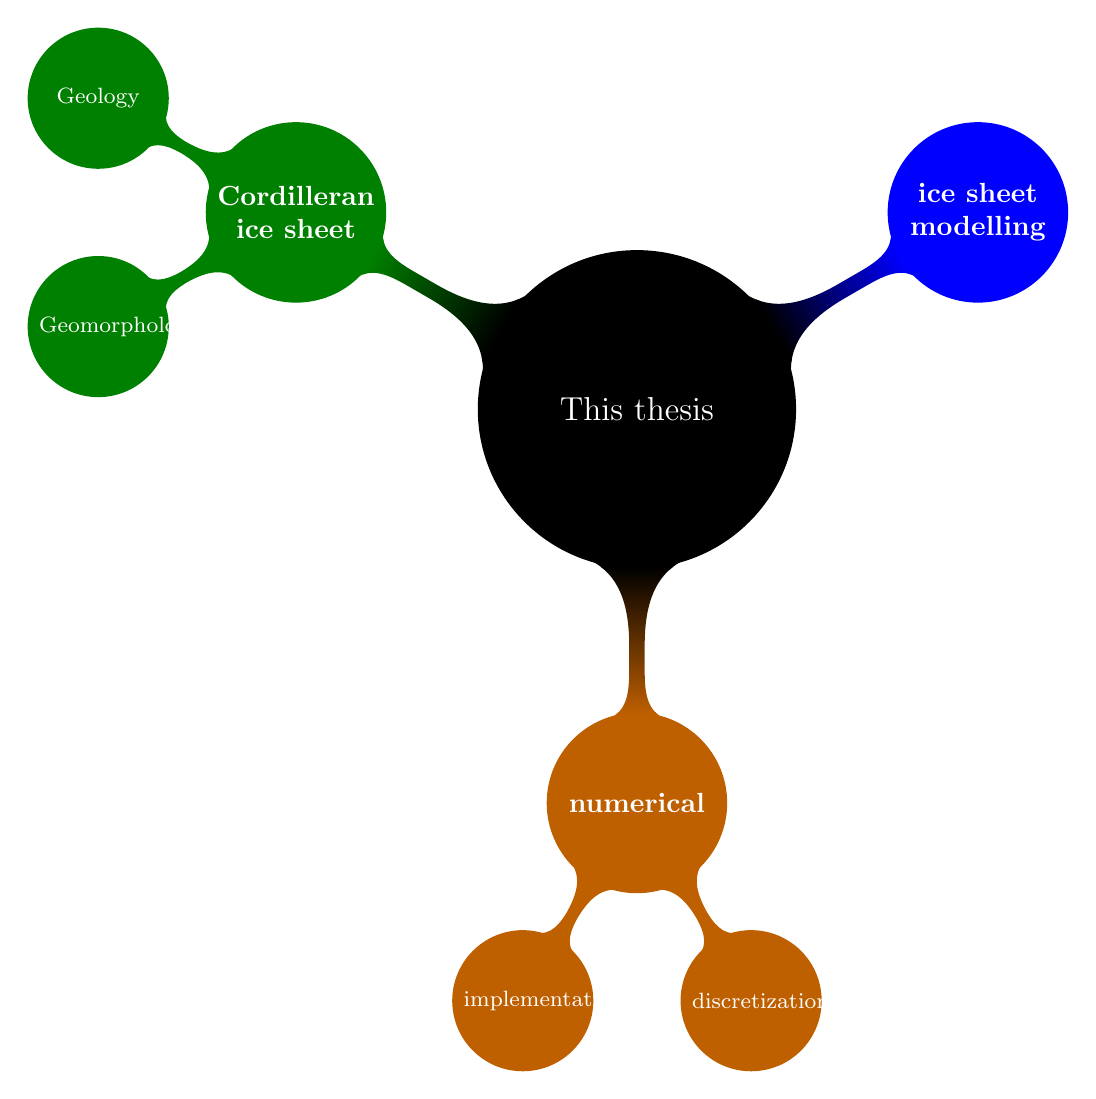
\begin{tikzpicture}
  \path[mindmap, grow cyclic, every node/.style=concept, concept color=black,text=white]
    node {This thesis}
    [clockwise from=150]
    child[concept color=green!50!black] { node {Cordilleran ice sheet}
      [clockwise from=210]
      child { node {Geomorphology} }
      child { node {Geology} }
    }  
    child[concept color=blue] { node {ice sheet modelling} }
    child[concept color=orange!75!black] { node {numerical}
      [clockwise from=-60]
      child { node {discretization} }
      child { node {implementation} }
    }
;
\end{tikzpicture}
\end{document}
